\begin{figure}[t]
    \centering
    \begin{tabular}{m{30mm} m{30mm} m{8mm}}
        \begin{minipage}[b]{\linewidth}
            \centering
            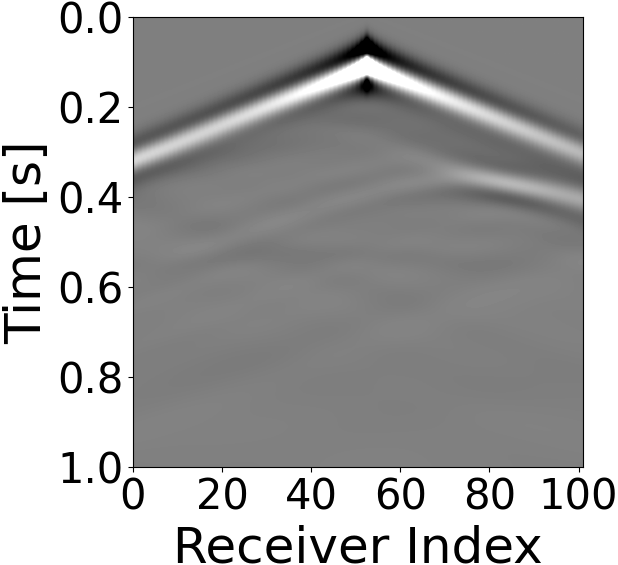
\includegraphics[width=\linewidth]{public/seismic_data}
            \vspace{-9mm}
            \caption*{\raisebox{-2mm}{\footnotesize Ground truth}}
            \vspace{1mm}
        \end{minipage} &
        \begin{minipage}[b]{\linewidth}
            \centering
            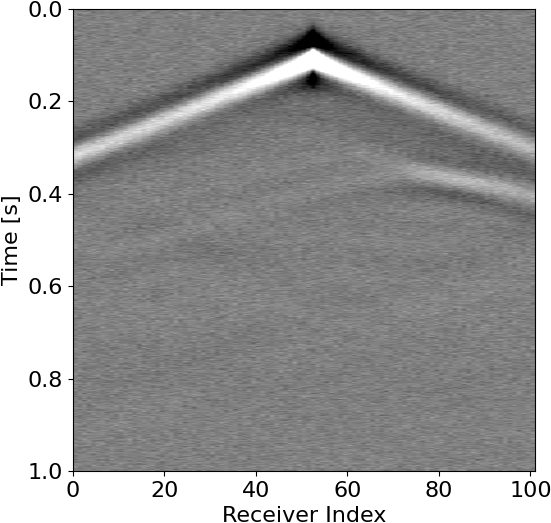
\includegraphics[width=\linewidth]{public/seismic_data_noisy}
            \vspace{-9mm}
            \caption*{\raisebox{-2mm}{\footnotesize Initial model}}
            \vspace{1mm}
        \end{minipage} &
        \multirow[t]{3}{*}{\raisebox{-5mm}{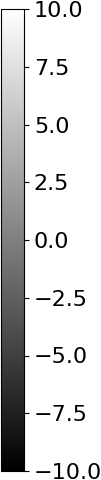
\includegraphics[height=20mm]{public/seismic-data-color-bar}}} \\
    \end{tabular}
    \vspace{-3mm}
    \caption{experiment-data}
    \label{fig:experiment-data}
\end{figure}
